\documentclass[12pt,oneside]{book} % for one-sided printing

\usepackage{blindtext}% Just used so we can generate some example text
\usepackage{amsmath}
\usepackage{amssymb}
\usepackage{mathtools}
\usepackage[export]{adjustbox}
\usepackage{lipsum}
\usepackage{booktabs}  % For better quality tables
\usepackage{tabularx}  % for the X column type
\usepackage{listings}
\usepackage{xcolor}
\usepackage{caption}
\usepackage{xfrac}
\usepackage{algorithmic}
\usepackage{indentfirst}
\usepackage{subcaption}
\usepackage{graphicx}
\usepackage{geometry}
\geometry{a4paper, margin=1in}

% Place style file after other packages.
\usepackage{cranfieldthesis}
\usepackage{lscape} % for landscape pages
\usepackage{float}
\usepackage[toc,title,page]{appendix}

% Couleurs personnalisées
\definecolor{backcolour}{rgb}{0.96, 0.96, 0.96} % Fond très clair
\definecolor{codegray}{rgb}{0.47, 0.47, 0.47}   % Commentaires et numéros de ligne
\definecolor{codegreen}{rgb}{0.25, 0.50, 0.35}  % Commentaires
\definecolor{codeblue}{rgb}{0.26, 0.44, 0.58}   % Mots-clés
\definecolor{codepurple}{rgb}{0.50, 0, 0.50}    % Identificateurs
\definecolor{codeteal}{rgb}{0, 0.5, 0.5}        % Chaînes de caractères
\definecolor{terminalback}{rgb}{0.05, 0.05, 0.05} % Fond très sombre pour le terminal
\definecolor{terminaltext}{rgb}{0.7, 0.7, 0.7}    % Texte clair pour le terminal

\lstdefinestyle{python}{
    language=Python,
    backgroundcolor=\color{backcolour},
    commentstyle=\color{codegreen},
    keywordstyle=\color{codeblue},
    numberstyle=\tiny\color{codegray},
    stringstyle=\color{codeteal},
    identifierstyle=\color{codepurple},
    basicstyle=\ttfamily\scriptsize,
    breakatwhitespace=false,
    breaklines=true,
    captionpos=b,
    keepspaces=true,
    numbers=left,
    numbersep=5pt,
    showspaces=false,
    showstringspaces=false,
    showtabs=false,
    tabsize=4,
    frame=single,
    rulecolor=\color{codegray},
    framexleftmargin=15pt,
    framextopmargin=5pt,
    framexbottommargin=5pt,
    framexrightmargin=15pt,
}

\lstdefinestyle{terminal}{
    backgroundcolor=\color{terminalback},
    basicstyle=\color{terminaltext}\ttfamily\scriptsize,
    frame=single,
    rulecolor=\color{codegray}, % Couleur grise pour le cadre
    framexleftmargin=15pt,
    framextopmargin=5pt,
    framexbottommargin=5pt,
    framexrightmargin=15pt,
    breaklines=true,
    captionpos=b,
    keepspaces=true,
    showspaces=false,
    showstringspaces=false,
    showtabs=false,
    tabsize=4,
    numbers=none,
}

% Title Page Set Up
\title{Machine learning \& Big Data Assignment}
\author{Alexis Balayre}
\date{20th November 2023}
\school{\SATM}
\degree{MSc}
\course{Computational Software of Techniques Engineering}
\academicyear{2023 - 2024}

% Supervisors
\supervisor{Dr Jun Li}

% Copyright
\copyrightyear{2023}

% References
\usepackage[numbers]{natbib} % for nice referencing
\makeatletter % Reference list option change to number and period
\renewcommand\@biblabel[1]{#1.} % from [1] to 1
\makeatother %
\setcitestyle{round} % use round citations

\begin{document}

\frontmatter

% Form Title Pages
\maketitle

% Use single spacing for Table of Contents, List of Figures, etc
{
    \clearpage
    \singlespacing
    % Table of Contents
    {
        \tableofcontents
    }
    \clearpage

    % List of Figures
    \listoffigures

    % List of Tables
    \listoftables
}

%% Main Matter
\mainmatter
\pagestyle{fancy}
\fancyhead[L]{\nouppercase{\leftmark}}
\fancyhead[R]{\nouppercase{\rightmark}}

\chapter{Introduction}
During the global COVID-19 pandemic, nations took advantage of Big Data
Analytics and Artificial Intelligence technologies to understand and combat the
spread of the virus. This report focuses on the detailed analysis of a
comprehensive global dataset of confirmed cases of COVID-19, leveraging Apache
Spark, an advanced data processing framework. The main objective is to provide
a clear picture of the evolution of the pandemic on a global scale. The aim is
to understand not only the speed and patterns of spread of the virus. It also
aims to demonstrate how Big Data tools can be used to transform, analyse and
interpret massive volumes of data, offering a unique and valuable perspective
in the management of global health crises.

\chapter{Dataset Description}

\subsection*{COVID-19 Dataset}

As shown in table~\ref{tab:covid19-dataset-sample}, the
``time\_series\_covid19\_confirmed\_global'' dataset presents each row with key
identifiers such as ``province/state'' and ``country/region'', as well as
geographical coordinates (latitude and longitude). Importantly, it traces the
progression of the pandemic since its inception, with each column dated in
mm/dd/yy format, revealing the total number of confirmed cases at that date.
This cumulative data structure enables a dynamic and detailed analysis of the
spread of the virus from 22 January 2020 to 9 March 2023. Moreover, the dataset
contains 201 distinct Countries/Regions, 92 distinct Provinces/States, and 198
null values for this last as shown in
tables~\ref{tab:covid19-dataset-distinct-values}
and~\ref{tab:covid19-dataset-null-values}.

\begin{table}[h!]
    \centering
    \captionsetup{font=large}
    \caption{COVID-19 Dataset Sample}
    \normalsize
    \begin{tabular}{|c|c|c|c|c|c|c|c|}
        \hline
          & Province/State & Country/Region & Lat       & Long      & 1/22/20 & \ldots & 3/9/23 \\
        \hline
        1 & NaN            & Afghanistan    & 33.93911  & 67.709953 & 0       &        & 209451 \\
        2 & NaN            & Albania        & 41.15330  & 20.168300 & 0       &        & 334457 \\
        3 & NaN            & Algeria        & 28.03390  & 1.659600  & 0       &        & 271496 \\
        4 & NaN            & Andorra        & 42.50630  & 1.521800  & 0       &        & 47890  \\
        5 & NaN            & Angola         & -11.20270 & 17.873900 & 0       &        & 105288 \\
        \hline
    \end{tabular}\label{tab:covid19-dataset-sample}
\end{table}

\begin{table}[h!]
    \centering
    \captionsetup{font=large}
    \caption{COVID-19 Dataset Statistics}
    \normalsize
    \begin{tabular}{|c|c|}
        \hline
        Column                  & Number of entries \\
        \hline
        Distinct Province/State & 92                \\
        Distinct Country/Region & 201               \\
        \hline
    \end{tabular}\label{tab:covid19-dataset-distinct-values}
\end{table}

\begin{table}[h!]
    \centering
    \captionsetup{font=large}
    \caption{COVID-19 Dataset Null Values}
    \normalsize
    \begin{tabular}{|c|c|}
        \hline
        Column         & Number of entries \\
        \hline
        Province/State & 198               \\
        Lat            & 2                 \\
        Long           & 2                 \\
        \hline
    \end{tabular}\label{tab:covid19-dataset-null-values}
\end{table}

\chapter{Methodologies}\label{chap:one}

\section{Queries Tasks}
\subsection{Query 1}

The first task is to calculate the average number of confirmed daily cases of
people infected with COVID-19 for each country in the dataset. This task is
implemented by the class \textbf{Query1} in Appendix~\ref{appendix:1}. The
steps of the task are as follows:
\begin{enumerate}
    \item \textbf{Pivoting the DataFrame:} The ``covidDataDf'' DataFrame initially contains dates in columns. This step reorganises the DataFrame so that the dates are row entries. It uses the stack function to transform each date column into a row, associated with its corresponding value. The result is a table with the following columns: ``Country/Region'', ``Date'' and ``Value''

    \item \textbf{Formatting Date Column:} The ``Date'' column is converted from a character string to an appropriate date format, in this case ``M/d/yy''.

    \item \textbf{Calculating Daily Cases:} A specification window separates the data by country and sorts it by date. Daily cases are calculated by subtracting the number of cases from the previous day from the current day's cases. The formula used is:
          \begin{equation}
              \text{DailyCases} =
              \begin{cases}
                  \text{0},                        & \text{if } \text{PrevValue is null} \\
                  \text{Value} - \text{PrevValue}, & \text{otherwise}
              \end{cases}
          \end{equation}
          where \texttt{PrevValue} is the number of cases from the previous day.

    \item \textbf{Grouping and Averaging Daily Cases:} The data is grouped by ``Country'', ``Year'' and ``Month''. For each group, the average number of cases per day is calculated. This gives the average number of confirmed cases per day for each month and country.
\end{enumerate}

\subsection{Query 2}

The second task is to calculate the mean, standard deviation, minimum and
maximum of the number of confirmed cases daily for each week and continent.
This task is implemented by the class \textbf{Query2} in
Appendix~\ref{appendix:2}. Here are the steps performed by the task:
\begin{enumerate}
    \item \textbf{Data Preparation (\texttt{\_\_prepare\_data method}):} The COVID data is prepared for analysis. A ``Location'' column is created by combining the values ``Province/State'' and ``Country/Region'' to consider the country if the state is not indicated.

    \item \textbf{Assigning Continents (\texttt{\_\_assign\_continent method}):} Continents are assigned to each line of data on the basis of geographical coordinates. To do this, the method uses the GeoPandas ``world\_boundaries\_gdf'' DataFrame, loaded from a shapefile~\cite{ContinentsBoundariesShapefile} containing continental boundaries, to identify the continent corresponding to a set of longitude and latitude coordinates. The method implements an internal determine\_continent function, which searches for the matching continent by checking whether a geographic point (formed by its coordinates) lies within the boundaries of one of the continents defined in ``world\_boundaries\_gdf''. If no match is found in this DataFrame, the method applies predefined geographic conditions~\cite{GISGeography2023} to approximate the continent. Finally, this logic is applied to each row of the covidDataDf DataFrame to add the new ``Continent'' column. This method was created using a GeoPandas Tutorial~\cite{DataCamp2023GeoPandas}.

    \item \textbf{Pivoting the DataFrame (\texttt{\_\_pivot\_table method}):} The ``covidDataDf'' DataFrame initially contains dates in columns. This step reorganises the DataFrame so that the dates are row entries. It uses the stack function to transform each date column into a row, associated with its corresponding value. The result is a table with the following columns: ``Location'', ``Continent'', ``Date'' and ``Value''

    \item \textbf{Computing Daily Confirmed Cases (\texttt{\_\_compute\_daily\_confirmed\_cases method}):} A window specification partitions the data by ``Location'' and orders it by ``Date''. Daily confirmed cases are calculated using the formula:
          \begin{equation}
              \text{DailyCases} =
              \begin{cases}
                  \text{0},                        & \text{if } \text{PrevValue is null} \\
                  \text{Value} - \text{PrevValue}, & \text{otherwise}
              \end{cases}
          \end{equation}
          where \texttt{PrevValue} is the number of cases from the previous day.

    \item \textbf{Computing Slopes (\texttt{\_\_compute\_slopes method}):} This method computes the slopes of daily confirmed cases for each location, preparing the data for linear regression. The slope is calculated using the formula:
          \begin{equation}
              \text{DailySlope} = \frac{n(\sum xy) - (\sum x)(\sum y)}{n(\sum x^2) - {(\sum x)}^2}
          \end{equation}
          where:
          \begin{itemize}
              \item $x$ is the number of days since the start of the dataset.
              \item $y$ is the number of daily confirmed cases.
              \item $n$ is the number of observations.
          \end{itemize}

    \item \textbf{Filtering Top Affected Locations (\texttt{\_\_filter\_top\_affected method}):} The top 100 affected locations are identified based on the slope of daily confirmed cases. To do this, the data is grouped by location and the maximum slope is calculated for each group. The top 100 locations are then selected.

    \item \textbf{Aggregating Data (\texttt{\_\_aggregate method}):} For each entry, a new ``WeekRange'' column is added with the start and end dates of the week on which the day in the ``Date'' column falls. The DataFrame is then grouped by continent and week. Statistical measures like mean, standard deviation, minimum, and maximum of daily cases are calculated for each group.
\end{enumerate}

\subsection{Query 3}
The last task is to perfom KMeans clustering on the top 50 affected locations
(depending on the slope of monthly confirmed cases) for each month. This task
is implemented by the class \textbf{Query3} in Appendix~\ref{appendix:3}. Here
are the steps performed by the task:
\begin{enumerate}
    \item \textbf{Data Preparation (\texttt{\_\_prepare\_data method}):}  The COVID data is prepared for analysis. A ``Location'' column is created by combining the values ``Province/State'' and ``Country/Region'' to consider the country if the state is not indicated.

    \item \textbf{Pivoting the DataFrame (\texttt{\_\_pivot\_table method}):} The ``covidDataDf'' DataFrame initially contains dates in columns. This step reorganises the DataFrame so that the dates are row entries. It uses the stack function to transform each date column into a row, associated with its corresponding value. The result is a table with the following columns: ``Location'', ``Date'' and ``Value''

    \item \textbf{Computing Daily Confirmed Cases (\texttt{\_\_compute\_daily\_confirmed\_cases method}):} Daily confirmed cases are computed using the formula:
          \begin{equation}
              \text{DailyCases} =
              \begin{cases}
                  \text{0},                        & \text{if } \text{PrevValue is null} \\
                  \text{Value} - \text{PrevValue}, & \text{otherwise}
              \end{cases}
          \end{equation}
          where \texttt{PrevValue} is the number of cases from the previous day.

    \item \textbf{Computing Monthly Slopes (\texttt{\_\_compute\_monthly\_slopes method}):} The slopes of monthly confirmed cases for each location are computed using linear regression. The slope formula used is:
          \begin{equation}
              \text{MonthlySlope} = \frac{n(\sum xy) - (\sum x)(\sum y)}{n(\sum x^2) - {(\sum x)}^2}
          \end{equation}
          where:
          \begin{itemize}
              \item $x$ is the number of months since the start of the dataset.
              \item $y$ is the number of monthly confirmed cases.
              \item $n$ is the number of observations.
          \end{itemize}

    \item \textbf{Filtering Top Affected Locations (\texttt{\_\_filter\_top\_affected method}):} The top 50 affected locations are identified based on the slope of monthly confirmed cases. To do this, the data is grouped by location and the mean slope is calculated for each group. The top 50 locations are then selected.

    \item \textbf{Applying Custom Clustering (\texttt{\_\_apply\_custom\_clustering method}):} A custom KMeans algorithm is applied to cluster the locations based on their slopes. This source code was adapted from the following Medium article~\cite{KMeansCustom}.

    \item \textbf{Applying Clustering (\texttt{\_\_apply\_clustering method}):} The standard KMeans algorithm from Spark MLlib is used for clustering the locations.
\end{enumerate}

\newpage

\section{Queries Optimisation}
Once the 3 queries had been built, an optimisation step was carried out to
improve task execution time. This section will look at the various difficulties
encountered and how to overcome them.

\subsection{Common Performance Problems in Spark}
The five most common performance issues encountered in Apache Spark, known as
the 5 Ss~\cite{ApacheSparkOptimizationTechniques} are:
\begin{enumerate}
    \itemindent=17.87pt
    \item \textbf{Spill:} When there is not enough RAM memory to process the current data,  Spark is forced to move some data to the hard disk, a process known as ``spilling''.
    \item \textbf{Skew:} The ``skew'' problem arises when data is not distributed evenly across partitions in Spark. Some nodes end up with a much heavier workload than others, creating bottlenecks and slowing down overall processing.
    \item \textbf{Shuffle:} During complex operations such as joins or clusters, Spark redistributes the data so that the corresponding elements are on the same node. Shuffling is costly in terms of performance because it involves intensive data transfer over the network.
    \item \textbf{Storage:} Inefficient storage management, such as processing many small files or using non-optimised file formats, can lead to a high number of I/O operations, which slows down performance. In addition, a poor storage strategy can also lead to shuffling and asymmetry problems.
    \item \textbf{Serialization:} ``Serialization'' i in Spark refers to the conversion of objects into a format that can be easily transmitted over the network or stored on disk. Inefficient serialization and deserialization processes can significantly slow down data transfer between cluster nodes and increase overall processing time.
\end{enumerate}

\subsection{Optimisation Solutions}
Here is a list of techniques for optimising Apache Spark processes and
overcoming performance problems~\cite{NNK2023}:
\begin{enumerate}
    \itemindent=17.87pt
    \item \textbf{Efficient partitioning:} Efficient partitioning in Apache Spark is essential for the balanced distribution of data across cluster nodes. This distribution plays a crucial role in optimising performance, particularly for shuffle operations. By adjusting the number of partitions with repartition() or coalesce(), it is possible to balance the workload between nodes, which is effective for join and aggregation operations, for example.
    \item \textbf{Persist/Cache and Early Filtering:} The judicious use of caching and early filtering goes hand in hand in optimising Spark processes. By using persist() or cache(), frequently accessed data is retained in memory, reducing the time required for repeated operations. At the same time, early data filtering, before resource-intensive operations such as joins or shuffles, can significantly reduce the amount of data processed, speeding up the whole process.
    \item \textbf{Data Format Choice:} The choice of data format is an often underestimated but crucial aspect of Spark optimisation. Columnar formats such as Parquet or ORC are preferable for efficient read and write operations. By choosing the right data format, you can significantly improve read performance and reduce the amount of storage space required.
    \item \textbf{Minimising Shuffle and Broadcast Operations:} Minimising shuffle operations is crucial to improving performance in Spark. Shuffles, which are necessary for operations such as joins and groupings, can be costly in terms of performance because they involve moving large amounts of data around the network. In addition, broadcasting is a powerful technique for joins involving a large table and a smaller table.
\end{enumerate}

\newpage

\section{Pipeline of the Project}
\subsection{Pipeline Overview}

The pipeline of this project is composed of four main components: \textbf{data
    ingestion}, \textbf{query 1}, \textbf{query 2} and \textbf{query 3}.\newline

The \textbf{ingestion} task retrieves the last version of the data set from the
source and stores it in the data lake (CSV file stored in local storage). Then,
the \textbf{queries 1, 2 \& 3} tasks retrieves the data from the data lake and
performs the queries on the data.

\begin{figure}[h]
    \centering
    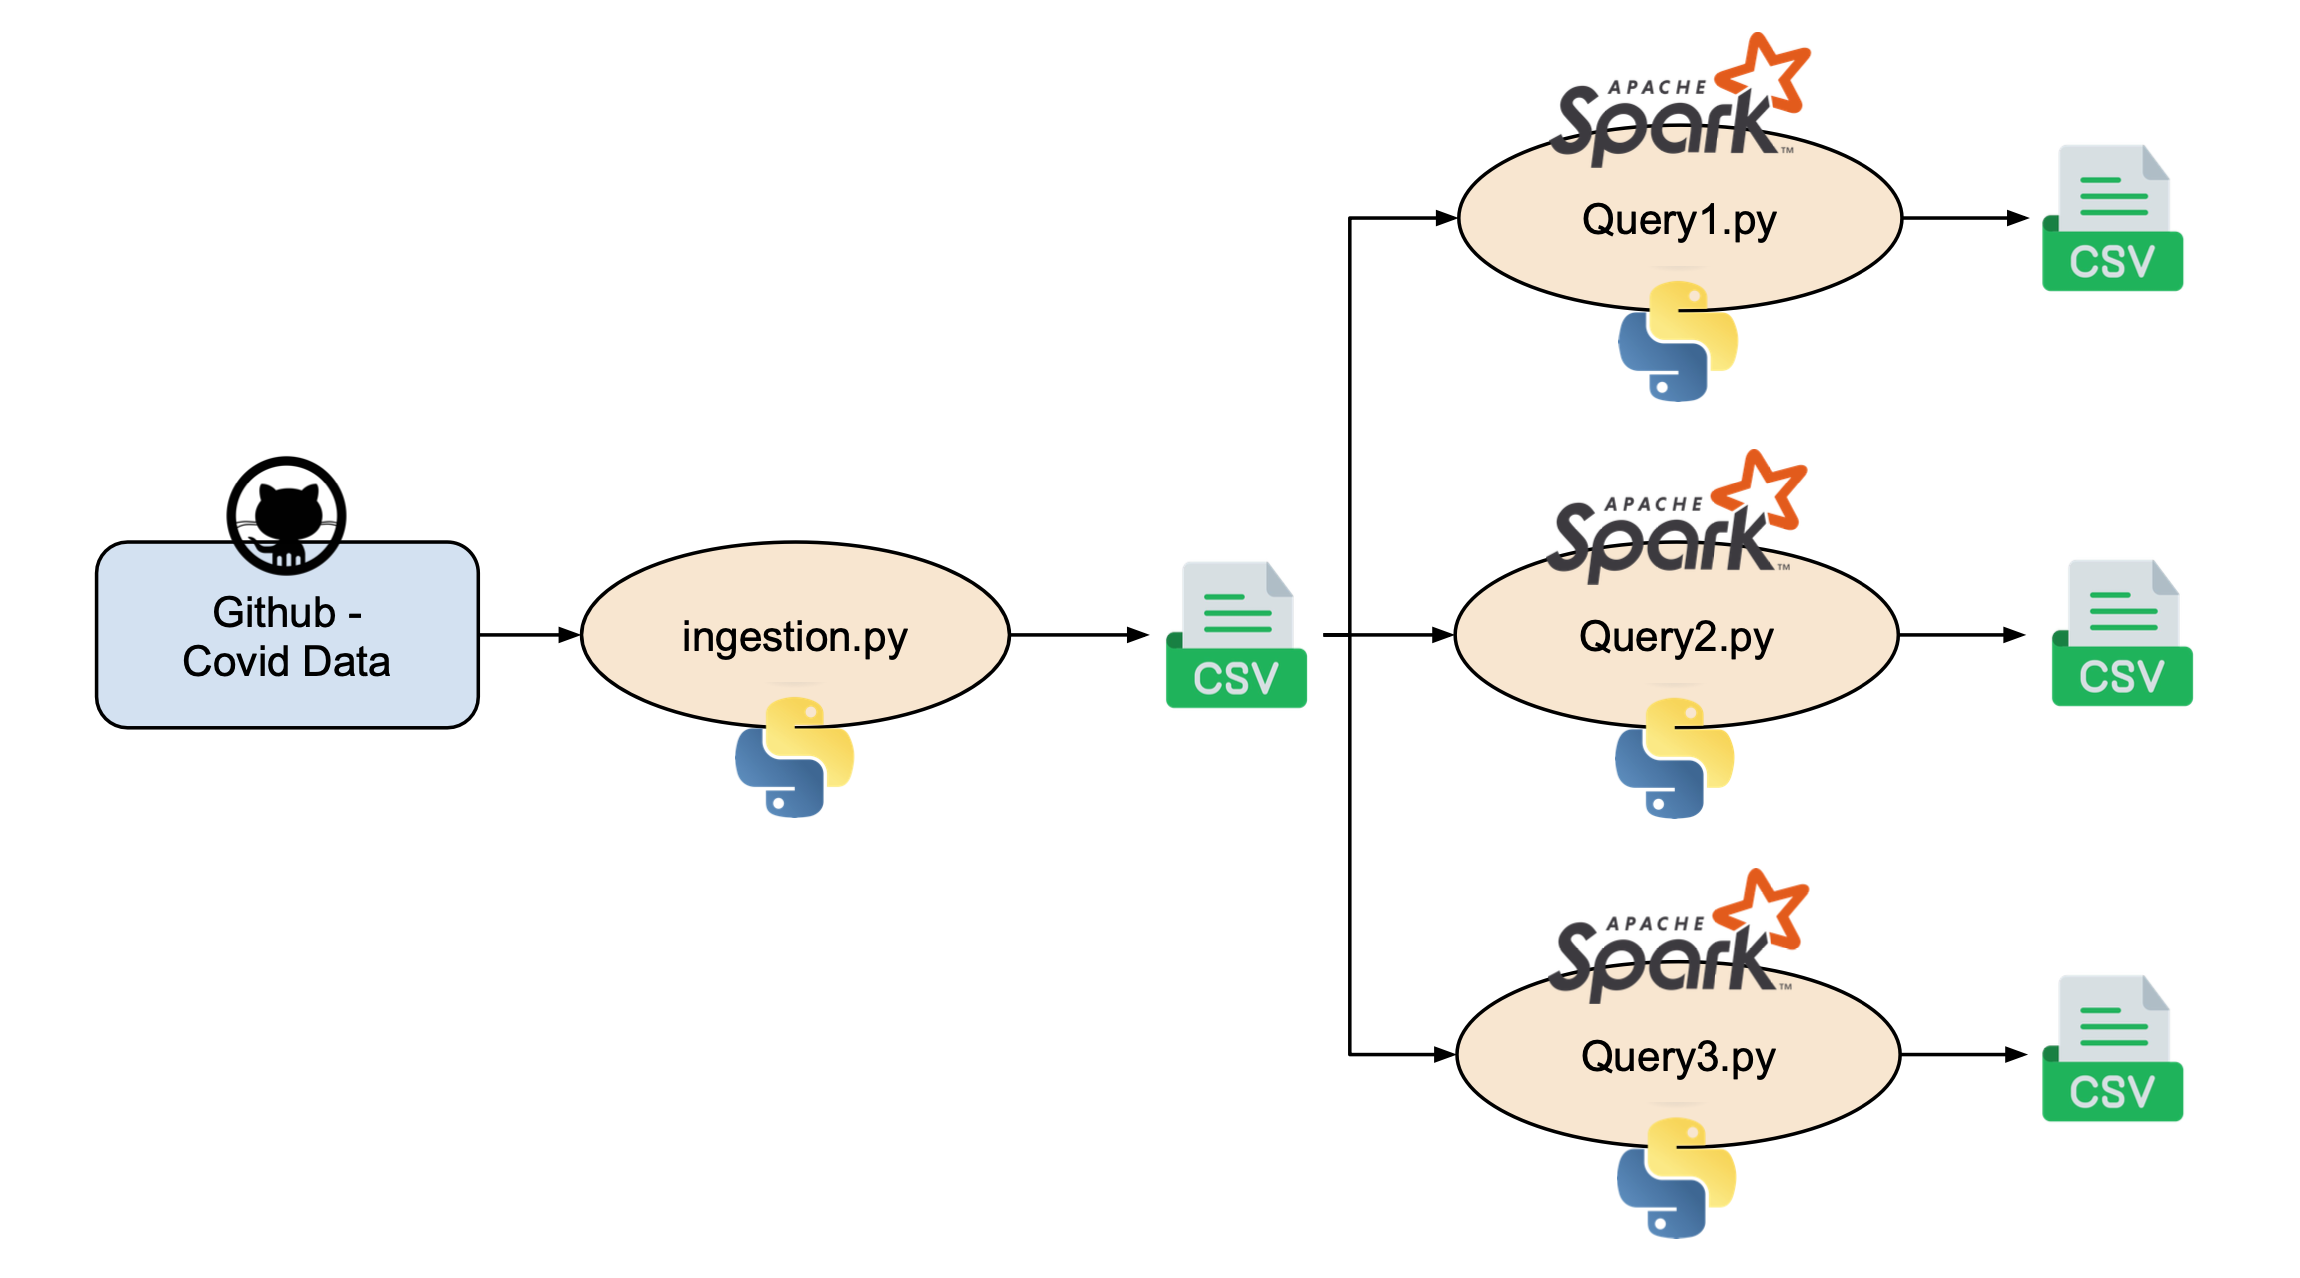
\includegraphics[width=1\linewidth]{images/pipeline.png}
    \caption{Pipeline Diagram}
\end{figure}

\newpage
\subsection{Pipeline Orchestration}

In order to orchestrate and automate the pipeline, a scheduled task must be run
every day to retrieve the latest version of the dataset and run the tasks when
a new daily row is added at 23:59 UTC to the dataset.\newline

To perform this task, a DAG (Directed Acyclic Graph) was created using Apache
Airflow. The DAG is scheduled to run every day at 00:00 UTC and is composed of
four tasks: \textbf{ingestion}, \textbf{query 1}, \textbf{query 2} and
\textbf{query 3}. The screenshot below~\ref{fig:apache-airflow} shows the DAG
graph of the pipeline in the web interface of Apache Airflow.\newline

The benefits of using a workflow platform such as Apache Airflow are its
ability to schedule and automate the pipeline, as well as its ability to
monitor the pipeline and send alerts if a task fails.

\begin{figure}[h]
    \centering
    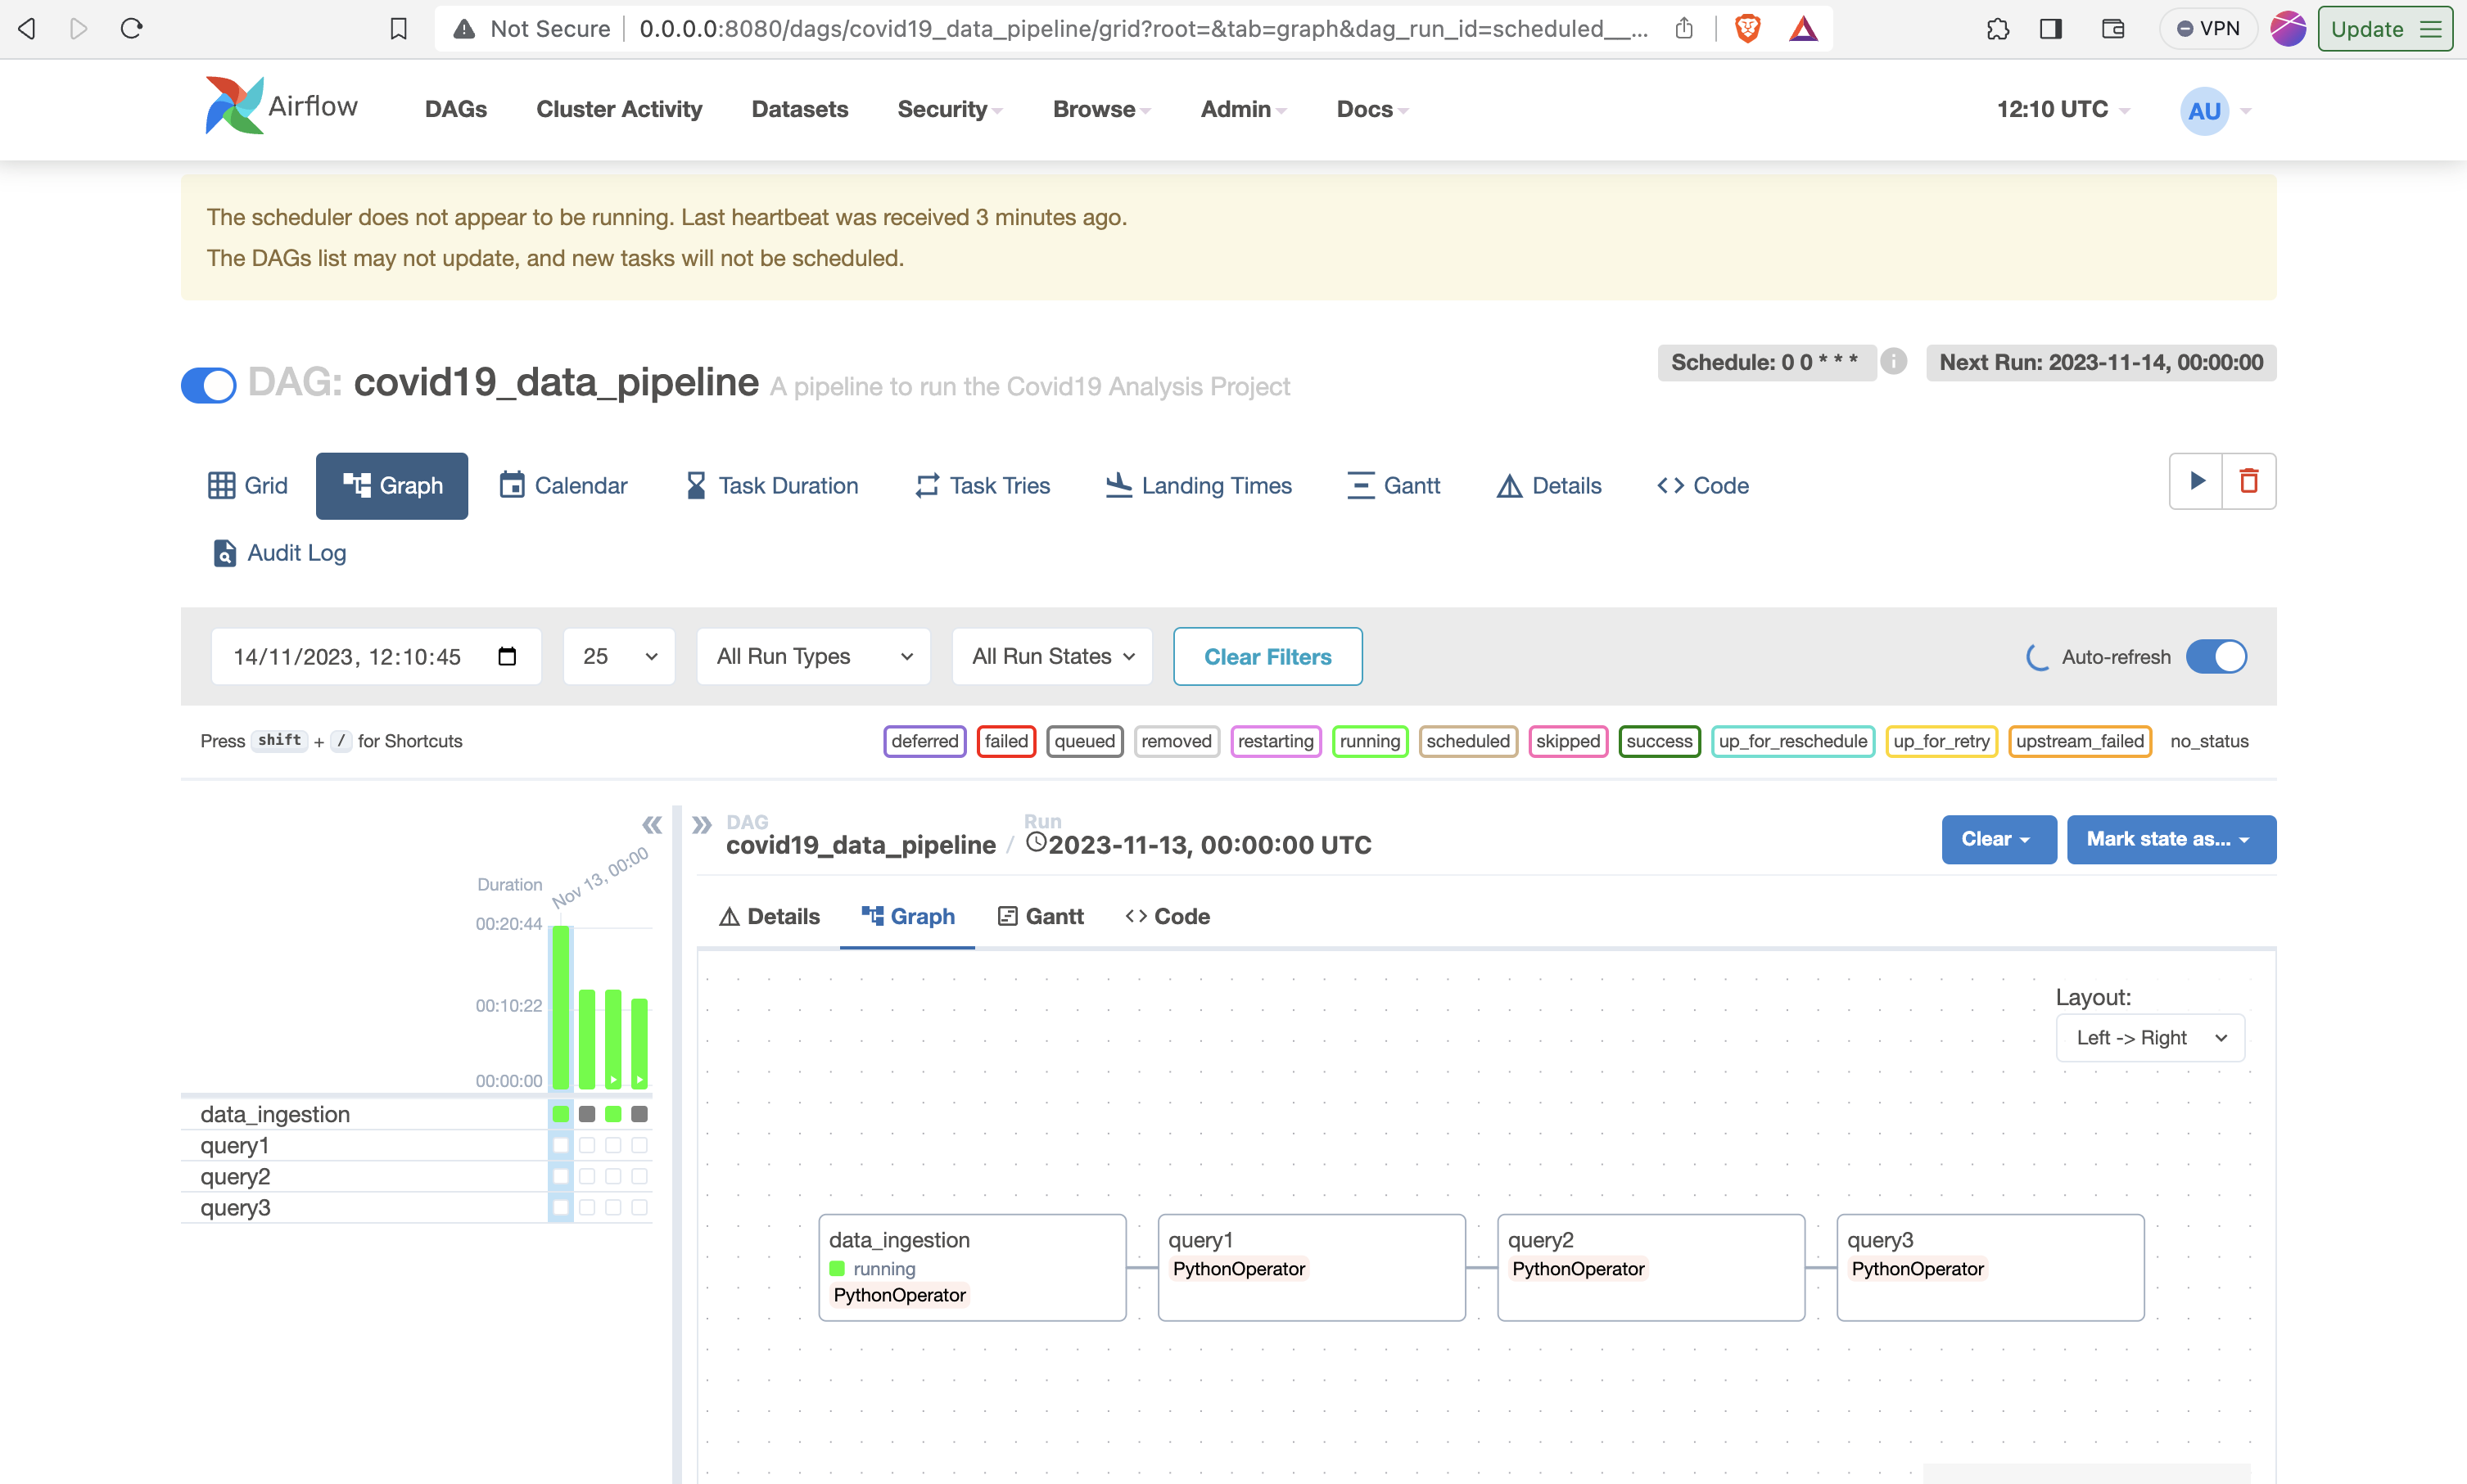
\includegraphics[width=1\linewidth]{images/Screenshot 2023-11-14 at 12.10.48.png}
    \caption{Apache Airflow DAG Graph}\label{fig:apache-airflow}
\end{figure}

\newpage
\chapter{Results \& Discussion}

\section{Queries Results}
The programme was last run on 18 November 2023. The appendix~\ref{appendix:4}
shows the output of the program on the terminal.

\subsection{Query 1}

The first query takes around 3 seconds, and the table
~\ref{tab:query1-results-sample} shows a sample of the data calculated during
the task. In order to evaluate performance, an equivalent script not using
Spark was run. Execution time was 0.5 sec. The~\ref{sec:discussion-of-results}
section will cover this point. The results are consistent with what was
expected~\cite{NYT}. For example, the figure~\ref{fig:sub1} shows that Brazil
was heavily impacted by the pandemic, reaching an average peak in February
2022. The same is true for Korea in figure~\ref{fig:sub2} and the United States
in figure~\ref{fig:sub3}, which were heavily impacted.

\begin{table}[h]
    \centering
    \captionsetup{font=large}
    \caption{Query 1 Results Sample}
    \normalsize
    \begin{tabular}{|l|c|c|c|c|c|}
        \hline
          & Country/Region & Year & Month & Average            \\
        \hline
        1 & Afghanistan    & 2020 & 1     & 0.0                \\
        2 & Afghanistan    & 2020 & 2     & 0.1724137931034483 \\
        3 & Afghanistan    & 2020 & 3     & 5.193548387096774  \\
        4 & Afghanistan    & 2020 & 4     & 55.36666666666667  \\
        5 & Afghanistan    & 2020 & 5     & 430.741935483871   \\
        \hline
    \end{tabular}\label{tab:query1-results-sample}
\end{table}

\begin{figure}[H]
    \vspace{-15pt}
    \centering
    \begin{subfigure}[b]{\linewidth}
        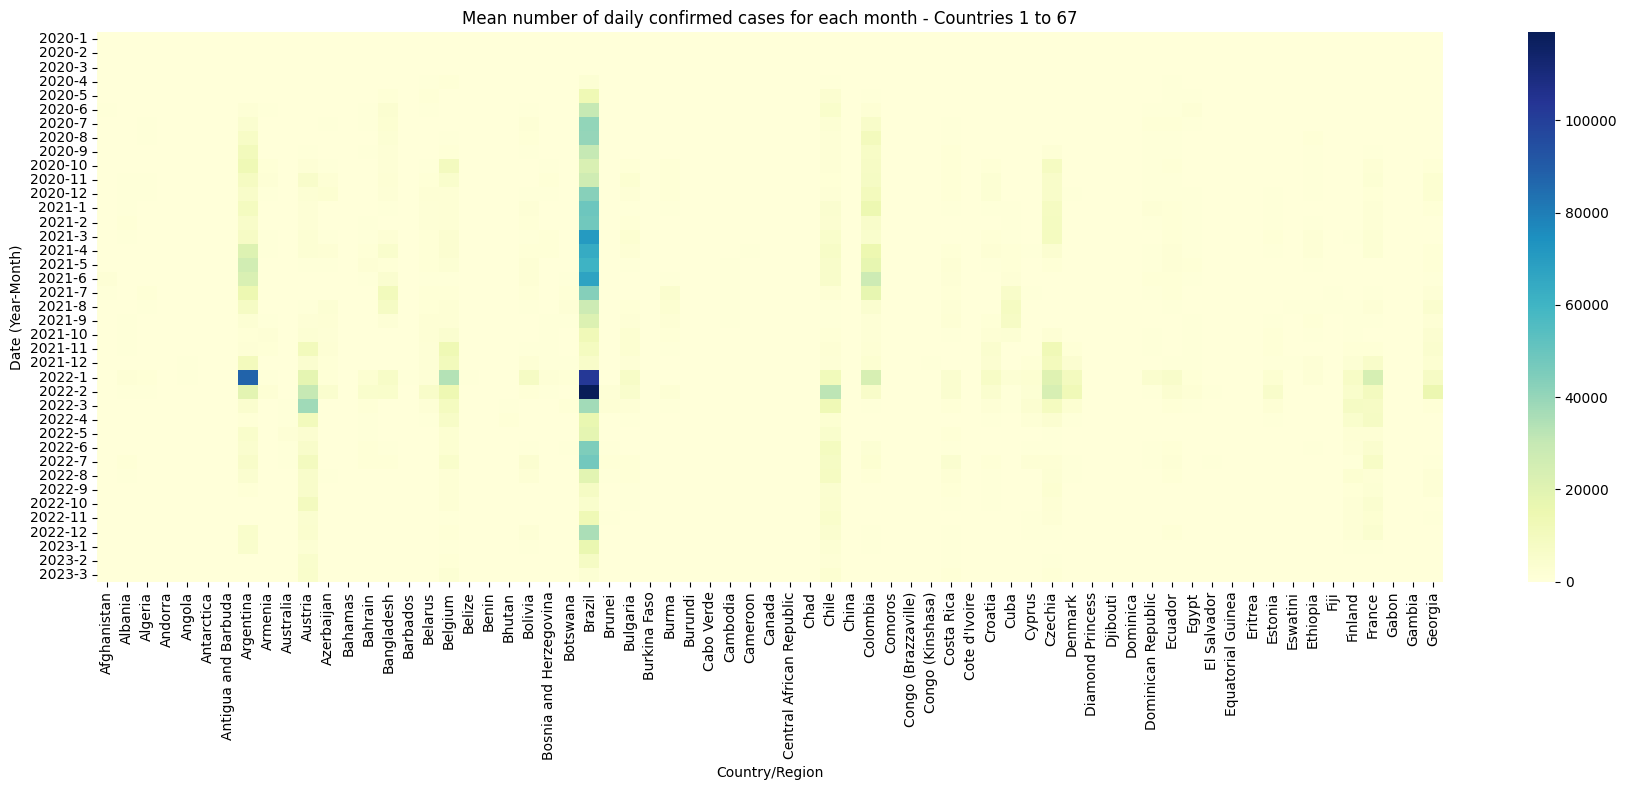
\includegraphics[width=\linewidth]{images/mean-daily-confirmed-cases-per-month-1.png}
        \caption{Countries 1 to 67}\label{fig:sub1}
        \vspace{-2pt}
    \end{subfigure}
    \hfill
    \begin{subfigure}[b]{\linewidth}
        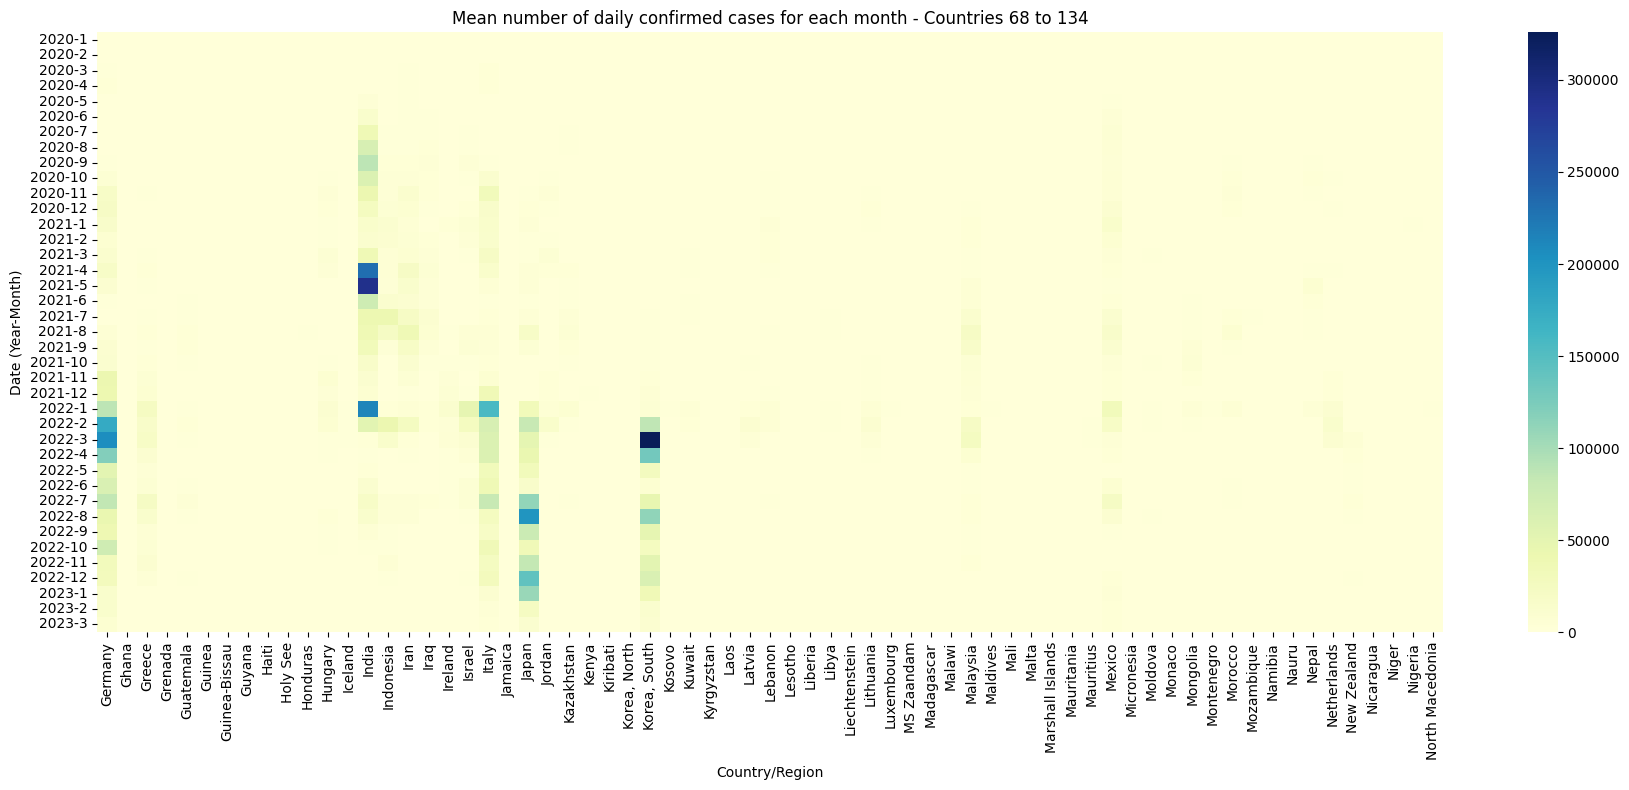
\includegraphics[width=\linewidth]{images/mean-daily-confirmed-cases-per-month-2.png}
        \caption{Countries 68 to 134}\label{fig:sub2}
        \vspace{-2pt}
    \end{subfigure}
    \hfill
    \begin{subfigure}[b]{\linewidth}
        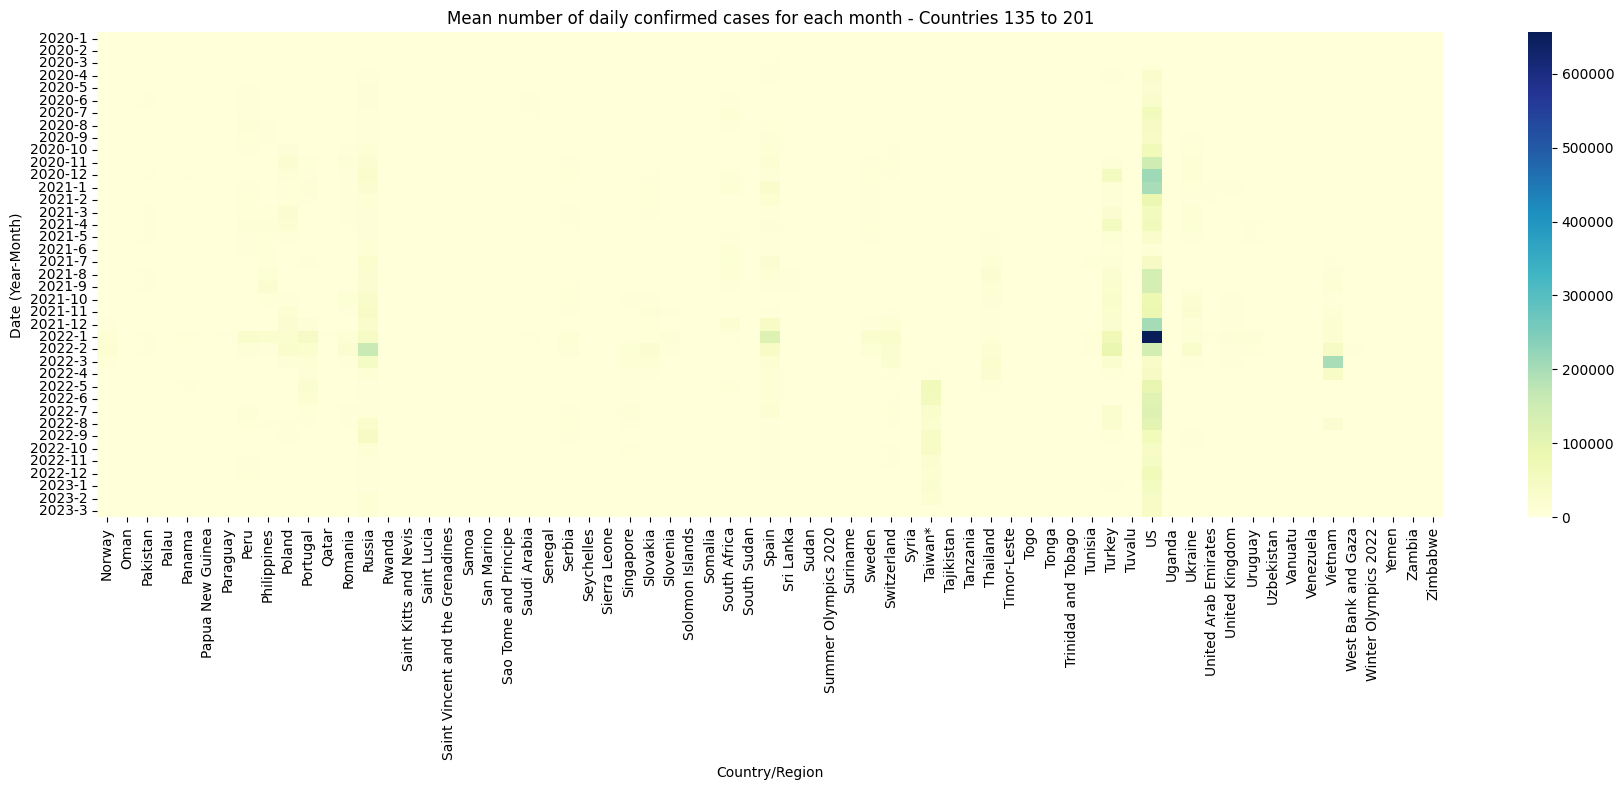
\includegraphics[width=\linewidth]{images/mean-daily-confirmed-cases-per-month-3.png}
        \caption{Countries 135 to 201}\label{fig:sub3}
        \vspace{-5pt}
    \end{subfigure}
    \caption{Mean Daily Confirmed Cases Per Month}\label{fig:mean-daily-confirmed-cases-per-month}
\end{figure}

\newpage
\subsection{Query 2}

The second query takes around 15 seconds, and the
table~\ref{tab:query2-results-sample} shows a sample of the data calculated
during the task. In order to evaluate performance, an equivalent script not
using Spark was run. Execution time was 6 sec.
The~\ref{sec:discussion-of-results} section will cover this point. Locations
used to compute the statistics are shown on the map of
figure~\ref{fig:top-100-locations-most-affected}. The area of the circles is
proportional to how the location has been affected by the pandemic.

\begin{figure}[H]
    \centering
    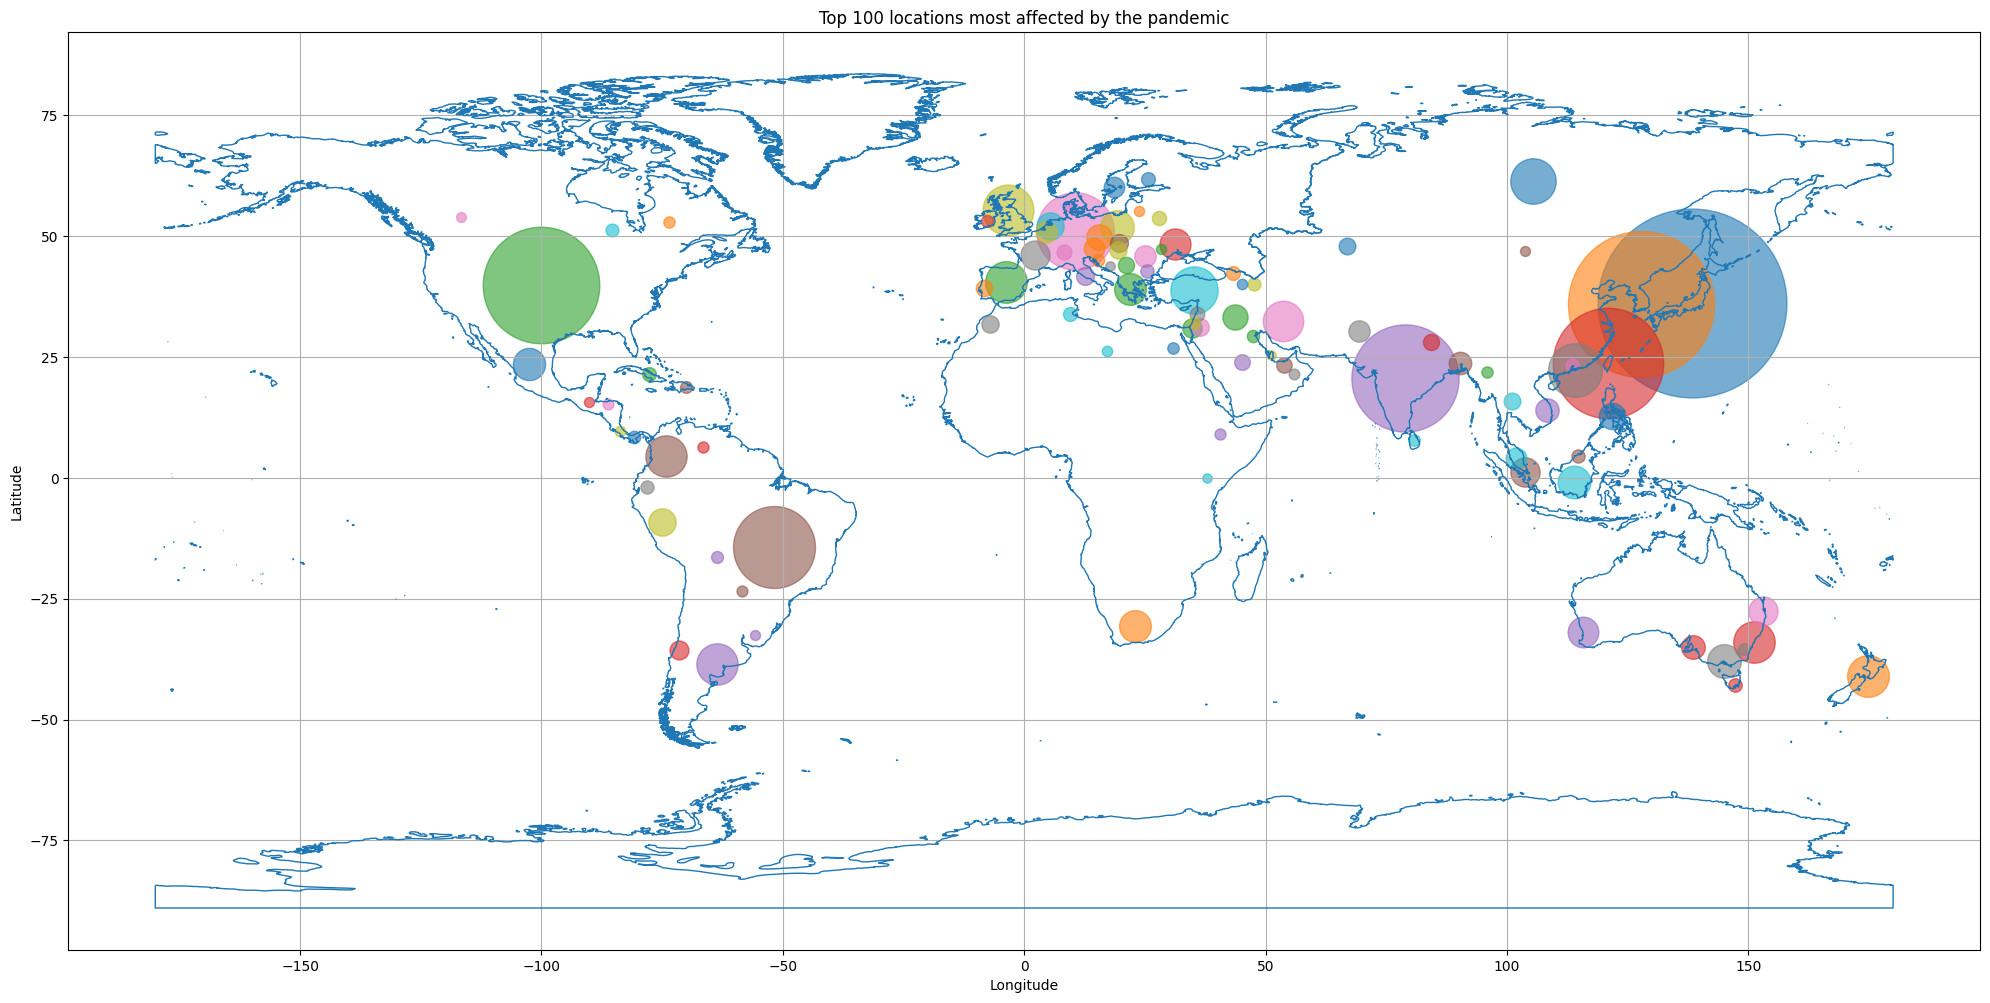
\includegraphics[width=1\linewidth]{images/top-100-locations-most-affected.png}
    \caption{Top 100 Locations most affected by the pandemic}\label{fig:top-100-locations-most-affected}
\end{figure}

\begin{table}[H]
    \centering
    \captionsetup{font=large}
    \caption{Query 2 Results Sample}
    \normalsize
    \begin{tabular}{|l|c|c|c|c|c|c|c|}
        \hline
           & Continent & WeekRange             & Mean     & Std      & Min & Max \\
        \hline
        1  & Africa    & 19/01/2020-25/01/2020 & 0.0      & 0.0      & 0   & 0   \\
        2  & Africa    & 26/01/2020-01/02/2020 & 0.0      & 0.0      & 0   & 0   \\
        3  & Africa    & 02/02/2020-08/02/2020 & 0.0      & 0.0      & 0   & 0   \\
        4  & Africa    & 09/02/2020-15/02/2020 & 0.0      & 0.0      & 0   & 0   \\
        5  & Africa    & 16/02/2020-22/02/2020 & 0.0      & 0.0      & 0   & 0   \\
        6  & Africa    & 23/02/2020-29/02/2020 & 0.0      & 0.0      & 0   & 0   \\
        7  & Africa    & 01/03/2020-07/03/2020 & 0.02857  & 0.16903  & 0   & 1   \\
        8  & Africa    & 08/03/2020-14/03/2020 & 0.65714  & 1.73108  & 0   & 9   \\
        9  & Africa    & 15/03/2020-21/03/2020 & 2.74285  & 4.53964  & 0   & 17  \\
        10 & Africa    & 22/03/2020-28/03/2020 & 12.62857 & 15.33754 & 0   & 59  \\
        11 & Africa    & 29/03/2020-04/04/2020 & 14.97142 & 19.31242 & 0   & 82  \\
        \hline
    \end{tabular}\label{tab:query2-results-sample}
\end{table}

\newpage

The figures below~\ref{fig:mean-confirmed-cases-by-week-and-continent}
and~\ref{fig:std-confirmed-cases-by-week-and-continent} show the mean and
standard deviation of the number of confirmed cases by week and continent. The
results are consistent with expectations: the continents most affected are
America and Europe~\cite{NYT}.

\begin{figure}[H]
    \centering
    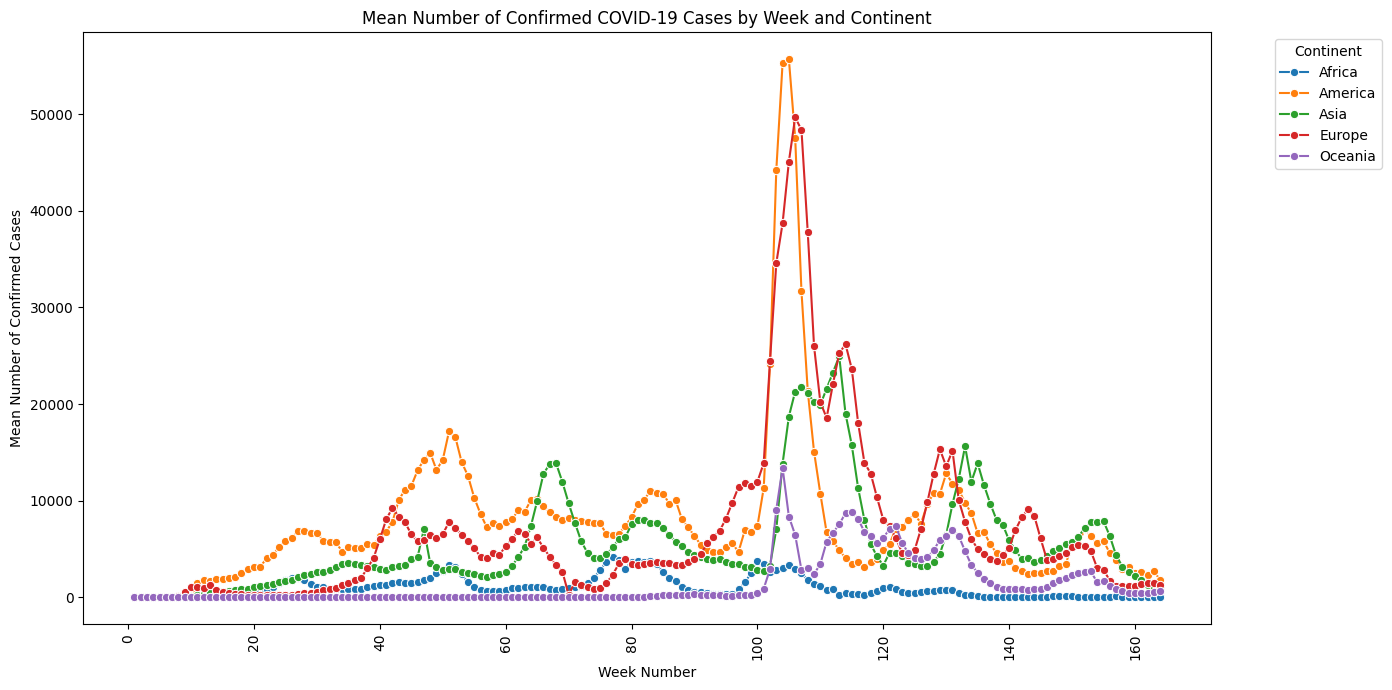
\includegraphics[width=1\textwidth]{images/mean-confirmed-cases-by-week-and-continent.png}
    \caption{Mean Confimed Cases By Week and Continent}\label{fig:mean-confirmed-cases-by-week-and-continent}
\end{figure}

\begin{figure}[H]
    \centering
    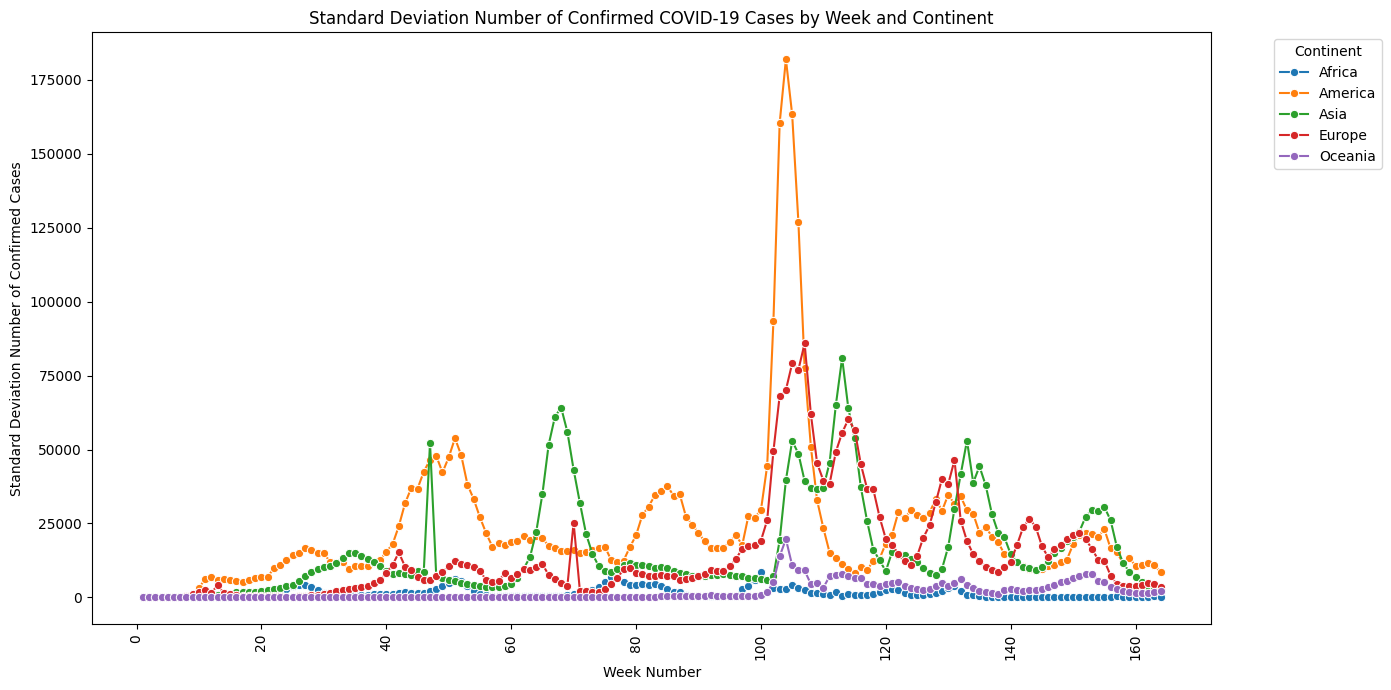
\includegraphics[width=1\textwidth]{images/std-confirmed-cases-by-week-and-continent.png}
    \caption{Standard Deviation Confimed Cases By Week and Continent}\label{fig:std-confirmed-cases-by-week-and-continent}
\end{figure}

\newpage
The figures~\ref{fig:max-confirmed-cases-by-week-and-continent} and~\ref{fig:min-confirmed-cases-by-week-and-continent} show the maximum and minimum of the number of confirmed cases by week and continent.

\begin{figure}[H]
    \centering
    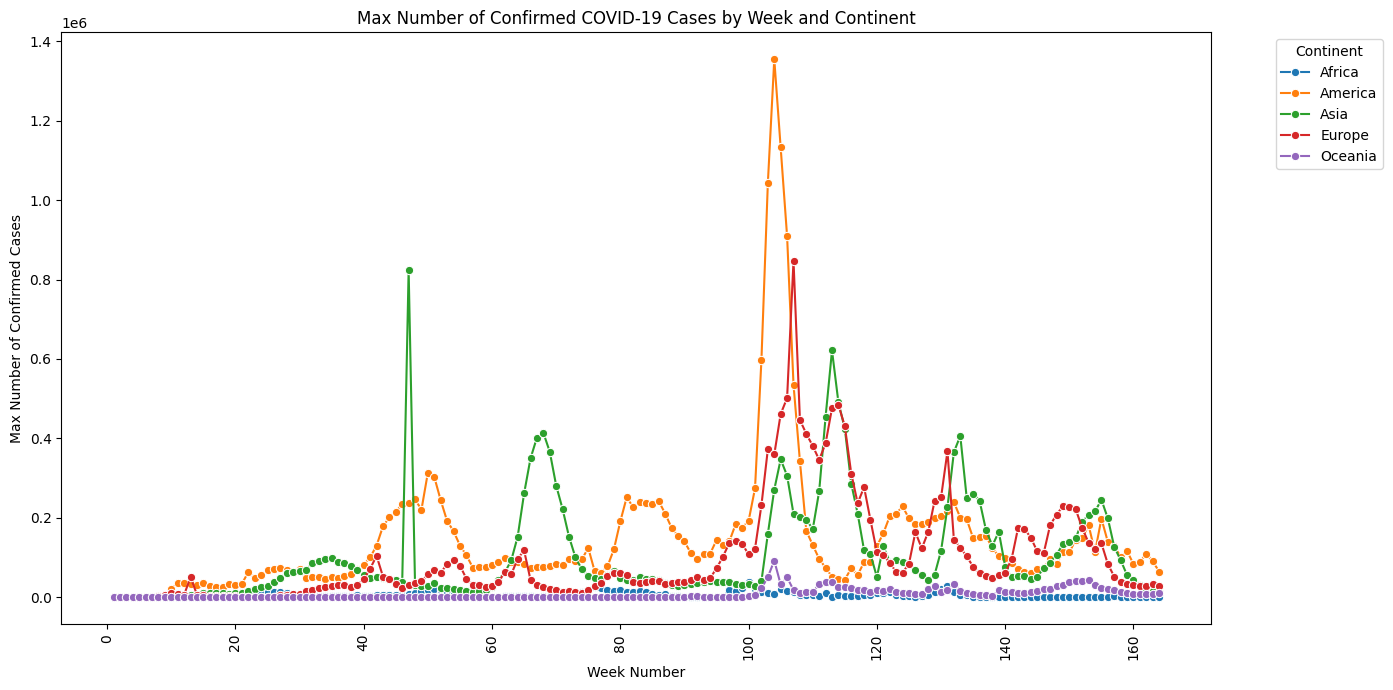
\includegraphics[width=1\textwidth]{images/max-confirmed-cases-by-week-and-continent.png}
    \caption{Maximum Confimed Cases By Week and Continent}\label{fig:max-confirmed-cases-by-week-and-continent}
\end{figure}

\begin{figure}[H]
    \centering
    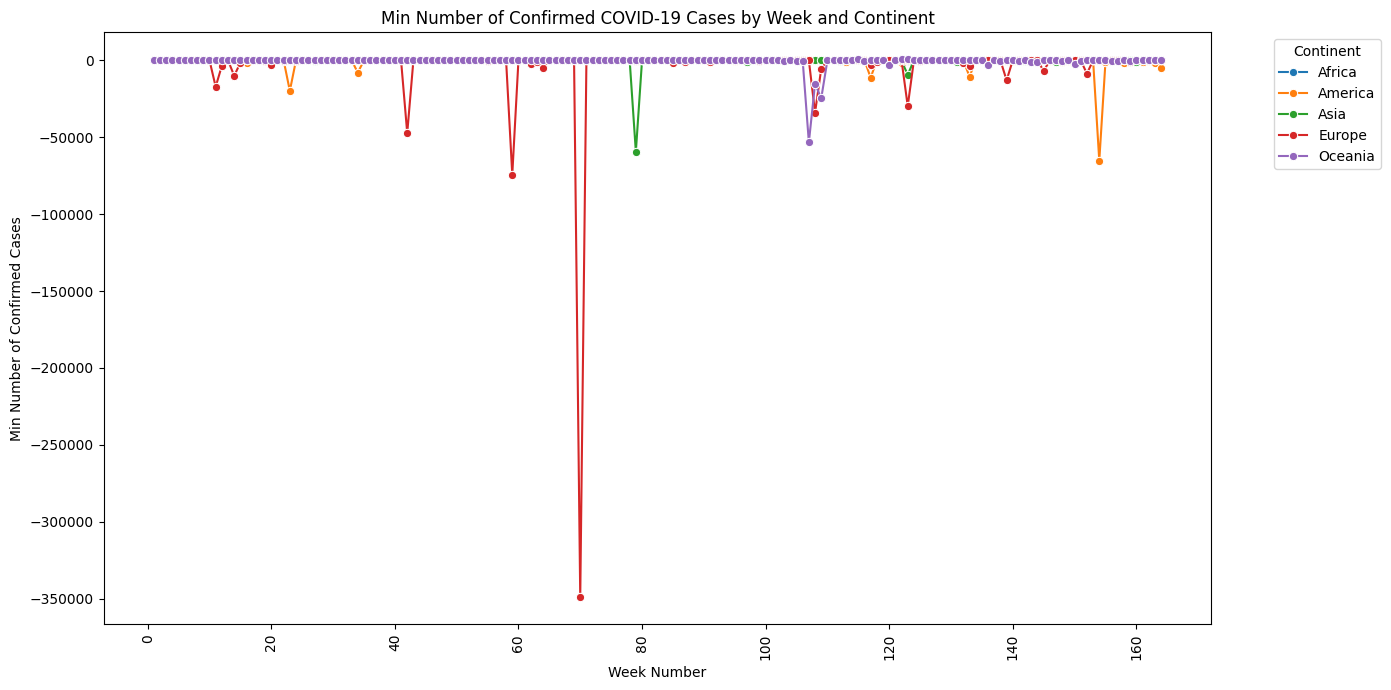
\includegraphics[width=1\textwidth]{images/min-confirmed-cases-by-week-and-continent.png}
    \caption{Minimum Confimed Cases By Week and Continent}\label{fig:min-confirmed-cases-by-week-and-continent}
\end{figure}

\newpage
\subsection{Query 3}

The third query takes around 3 minutes as clustering with the custom
implementation takes 60 seconds and clustering with the Spark MLlib
implementation takes 110 seconds. The
table~\ref{tab:query3-custom-results-sample} shows a sample of the data
calculated during the task with the custom implementation and the
table~\ref{tab:query3-spark-results-sample} with the Spark MLlib
implementation. Locations used to compute the statistics are shown on the map
of figure~\ref{fig:top-50-locations-most-affected}. The area of the circles is
proportional to how the location has been affected by the pandemic.

\begin{figure}[H]
    \centering
    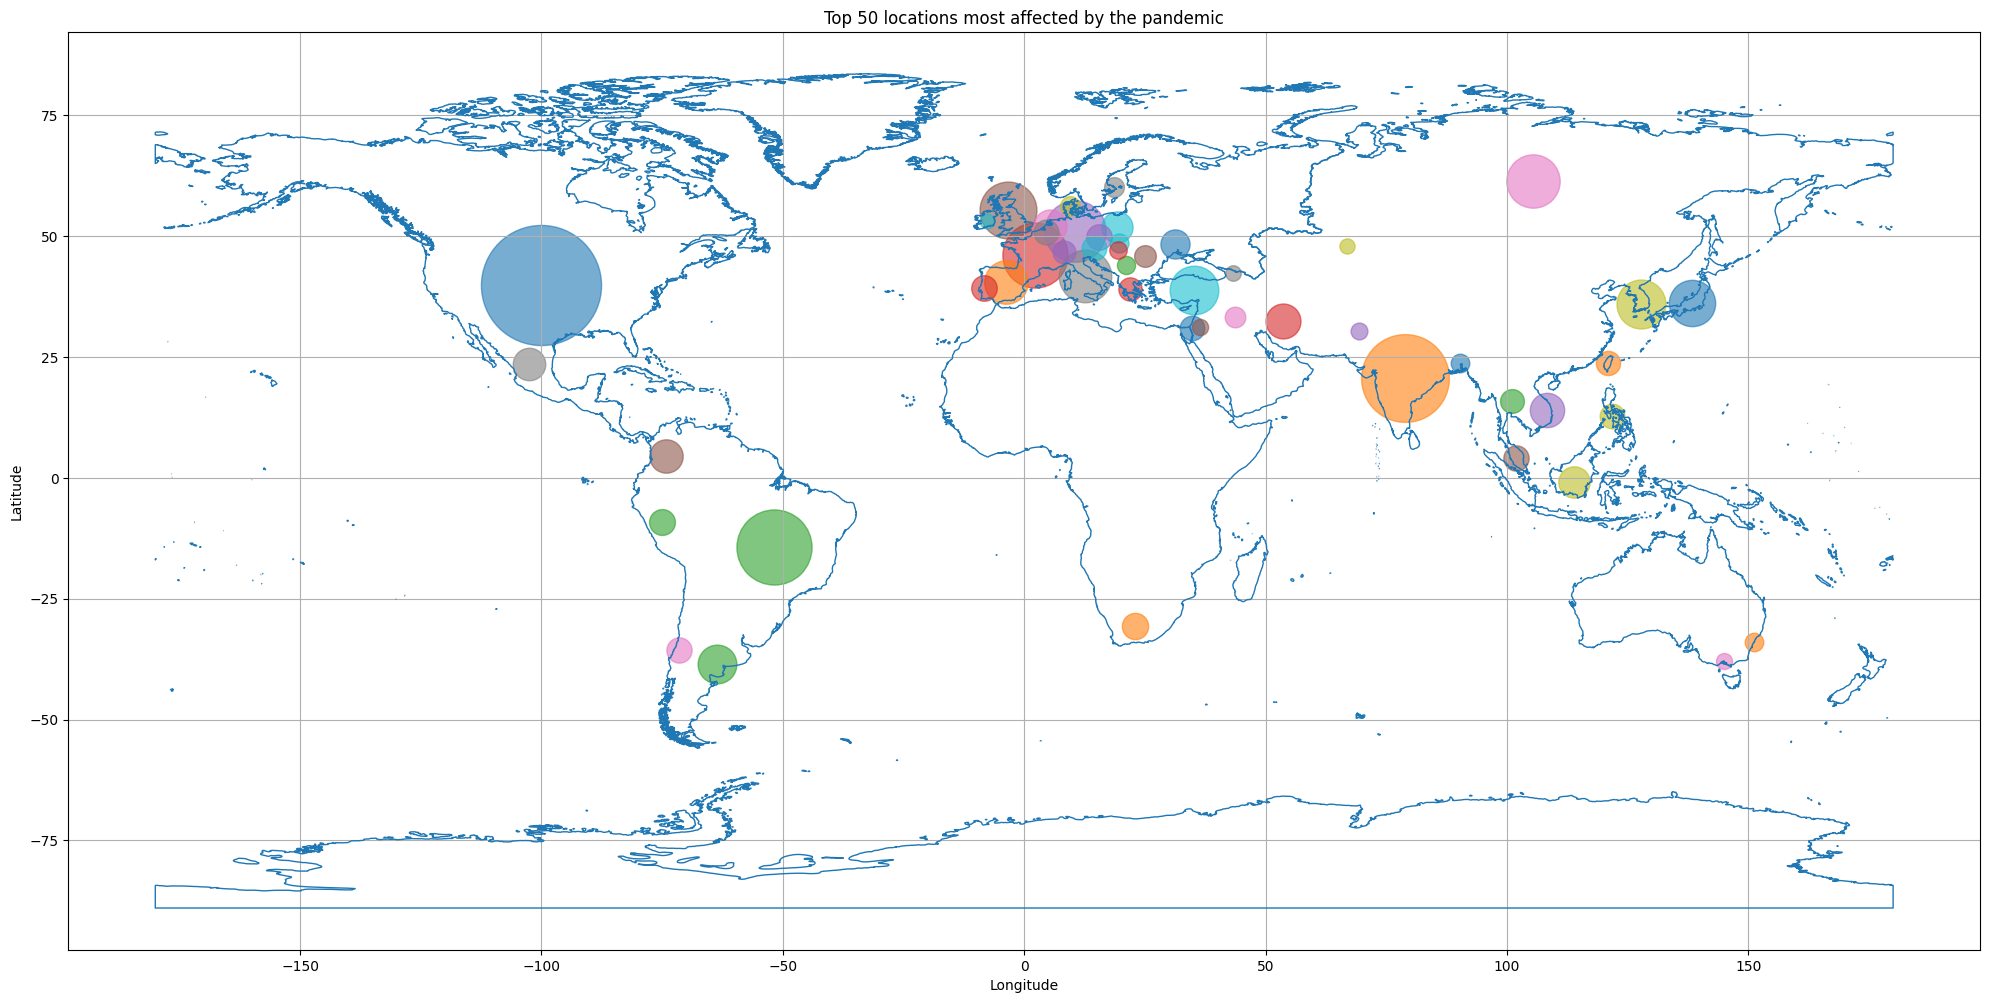
\includegraphics[width=1\linewidth]{images/top-50-locations-most-affected.png}
    \caption{Top 50 Locations most affected by the pandemic}\label{fig:top-50-locations-most-affected}
\end{figure}

\begin{table}[H]
    \centering
    \captionsetup{font=large}
    \caption{Query 3 Results Sample - Custom KMeans Clustering}
    \normalsize
    \begin{tabular}{|l|c|c|c|c|}
        \hline
          & Location  & Month   & Cluster \\
        \hline
        1 & Argentina & 2020-01 & 2       \\
        2 & Austria   & 2020-01 & 2       \\
        3 & Brazil    & 2020-01 & 2       \\
        4 & Czechia   & 2020-01 & 2       \\
        5 & France    & 2020-01 & 1       \\
        \hline
    \end{tabular}\label{tab:query3-custom-results-sample}
\end{table}

\begin{table}[H]
    \centering
    \captionsetup{font=large}
    \caption{Query 3 Results Sample - Spark MLlib KMeans Clustering}
    \normalsize
    \begin{tabular}{|l|c|c|c|c|}
        \hline
          & Location  & Month   & Cluster \\
        \hline
        1 & Argentina & 2020-01 & 2       \\
        2 & Austria   & 2020-01 & 0       \\
        3 & Brazil    & 2020-01 & 2       \\
        4 & Czechia   & 2020-01 & 2       \\
        5 & France    & 2020-01 & 1       \\
        \hline
    \end{tabular}\label{tab:query3-spark-results-sample}
\end{table}

\newpage

The figures below~\ref{fig:covid-19-clusters-custom}
and~\ref{fig:covid-19-clusters-spark} show the clusters of the top 50 locations
most affected by the pandemic in March 2020. The clusters are represented by
different colours.

\begin{figure}[H]
    \centering
    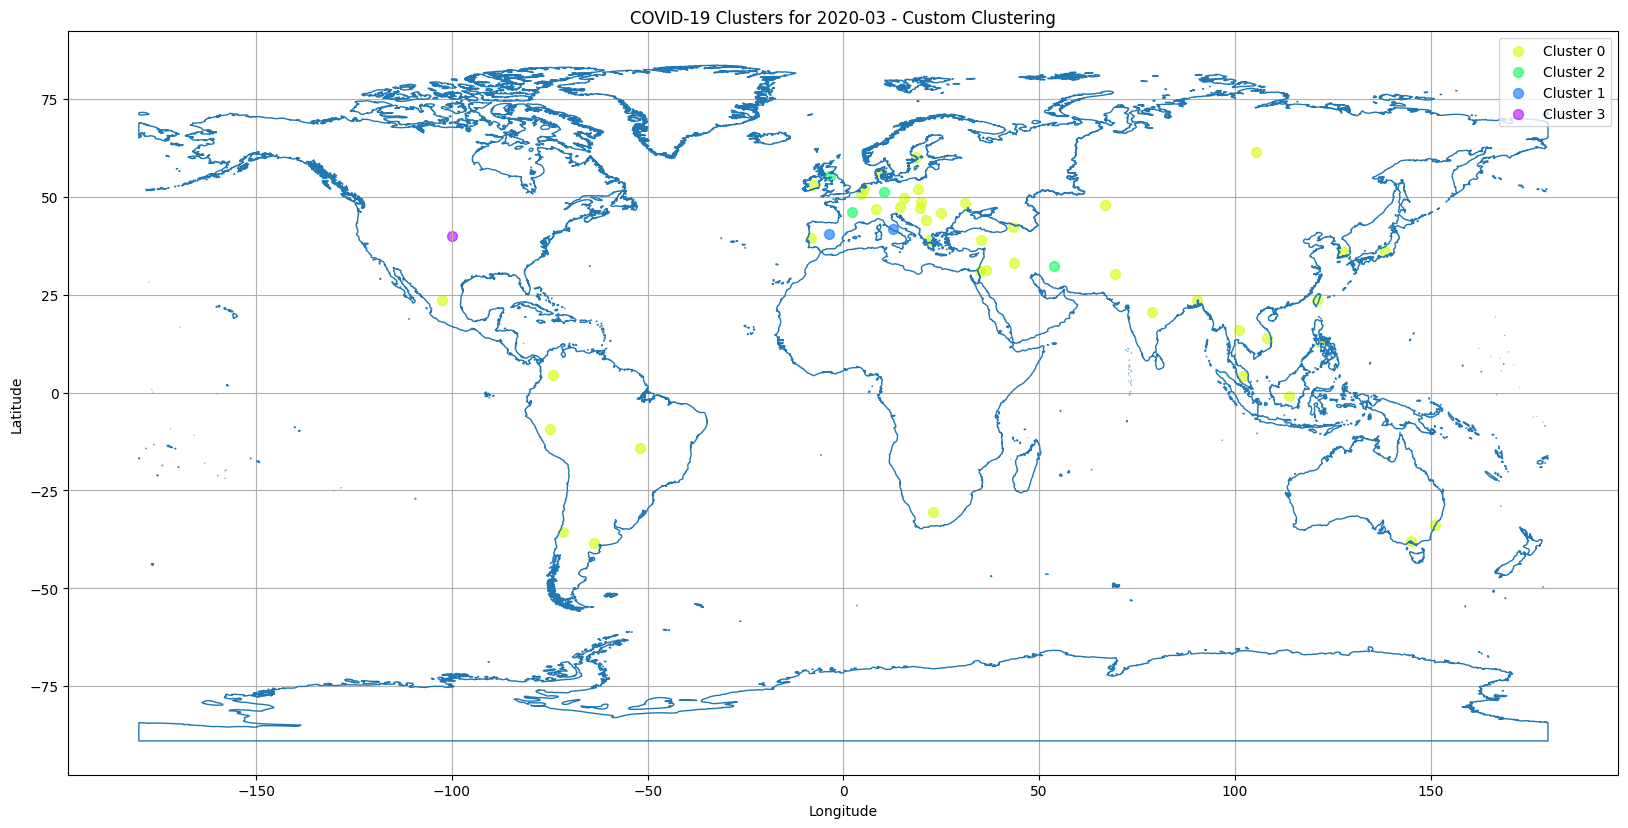
\includegraphics[width=1\textwidth]{images/covid-19-clusters-custom.png}
    \caption{Custom KMeans Clustering on 03/2020}\label{fig:covid-19-clusters-custom}
\end{figure}

\begin{figure}[H]
    \centering
    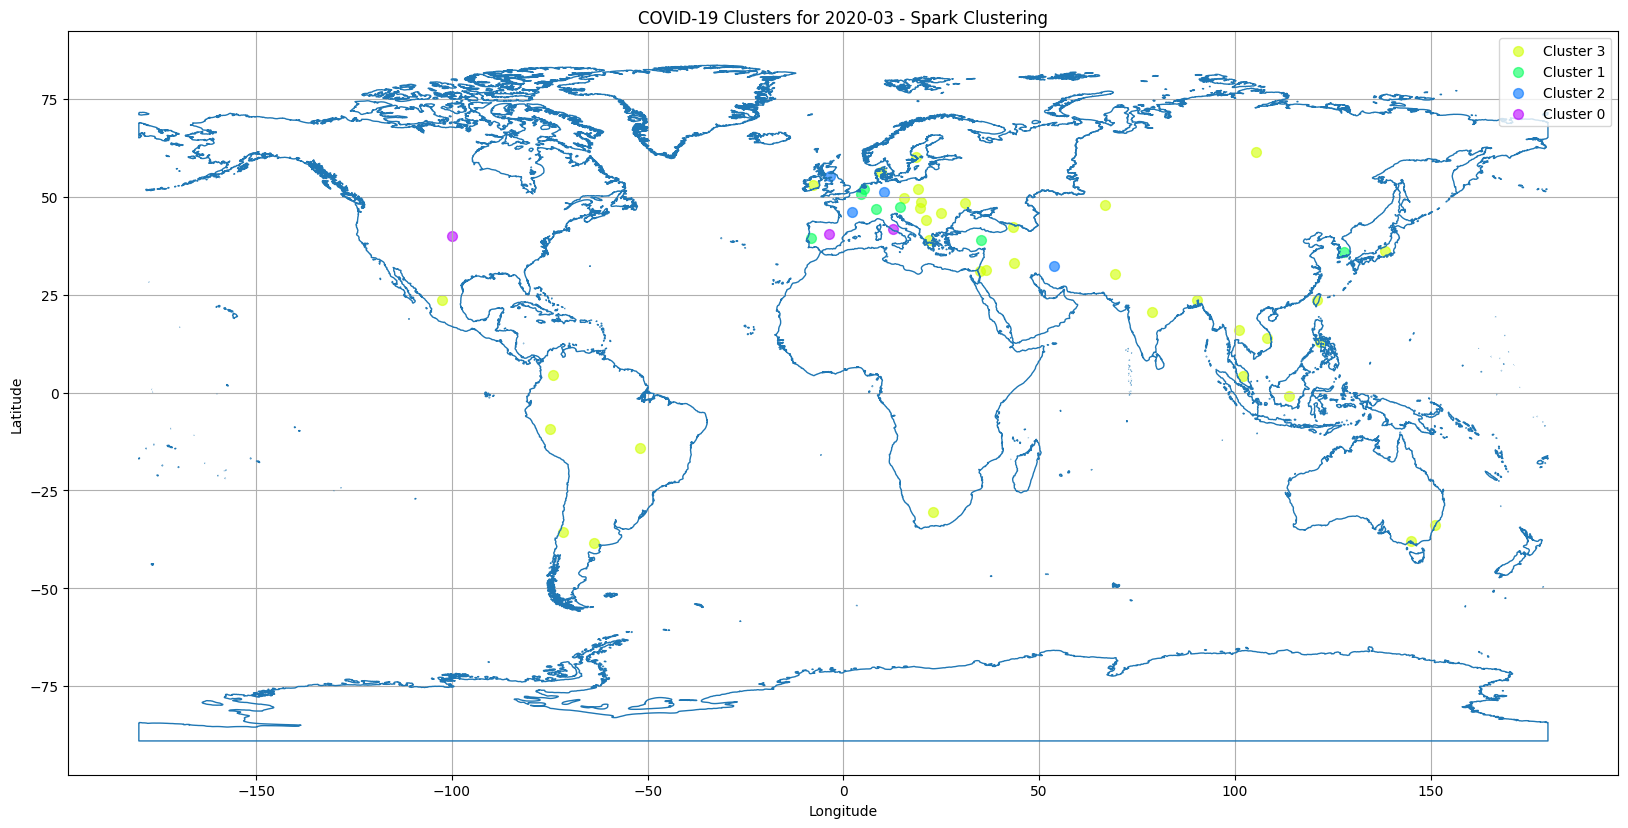
\includegraphics[width=1\textwidth]{images/covid-19-clusters-spark.png}
    \caption{Spark MLlib KMeans Clustering on 03/2020}\label{fig:covid-19-clusters-spark}
\end{figure}

\newpage

\section{Discussion of Results}\label{sec:discussion-of-results}
As the previous results show, it seems that scripts not using Spark are faster.
While these differences in execution time may seem surprising at first glance,
they can in fact be attributed to several factors:

\begin{enumerate}
    \item \textbf{Data size and structure:} The DataFrame, with its 289 entries and 1147 columns occupying 2.5 MB of memory, is relatively modest in size. Pandas is particularly efficient at processing such large amounts of data in memory on a single node. Spark, on the other hand, is designed for distributed processing of large datasets. In this case, the overheads of distributing the data and managing the Spark environment may outweigh the benefits of using it for smaller datasets.
    \item \textbf{Operational efficiency:} Pandas performs vectorised operations that are optimised for speed, especially with datasets that fit easily into memory on a single computer. Spark, while powerful for processing large volumes of data, introduces an initial overhead for distributing data and configuring the distributed environment, which can slow down processing for smaller datasets.
    \item \textbf{Complexity of the environment:} Complexity of the environment: Running operations in a Spark environment involves initializing a cluster (even in local mode), distributing tasks, and managing distributed memory, which adds extra processing time compared to running in-memory Pandas directly.
\end{enumerate}

Thus in this project run locally, Pandas is faster than Spark, due to its
efficient management of in-memory operations on a single node. Spark's
distributed processing overhead makes it less efficient for such tasks.

\newpage
\section{Ethical Considerations and Challenges}

In the context of the COVID-19 pandemic, the use of Machine Learning and Big
Data, while beneficial for crisis management, raises complex ethical issues and
challenges.\newline

Firstly, the management of health data, which is essential for tracking and
preventing the spread of the virus, creates major risks for privacy. preventing
the spread of the virus, creates major privacy risks. Massive data collection
and analysis can lead to intrusive surveillance, where the boundaries between
public security and individual privacy become blurred. This can constitute an
infringement of the right to privacy. In addition, some countries have taken
the opportunity to monitor their populations. For example, China has used
facial recognition technology to track people's movements and apply quarantine
measures.\newline

Secondly, algorithmic biases represent a major challenge. Machine learning
systems, although powerful, can incorporate and amplify existing biases in the
data. In the context of the pandemic, this could result in inequitable
distribution of medical resources, biased diagnoses or discriminatory public
health policies, disproportionately affecting certain social or ethnic
groups.\newline

Thirdly, transparency and accountability are crucial issues. Complex and often
opaque algorithms make it difficult to understand and challenge AI-based
decisions. This raises questions of governance and regulation: who is
responsible for errors or harm caused by automated decisions? How can these
technologies be effectively controlled and regulated?\newline

Finally, there is the overall challenge of striking a balance between the
benefits of using these technologies and respect for fundamental rights.
Striking the right balance between effective management of the pandemic and
protection of individual freedoms is a delicate exercise, requiring careful
ethical reflection and judicious regulation.

\newpage
\chapter{Conclusion}

This study demonstrated the effectiveness of Big Data and Machine Learning
technologies in the analysis and management of the COVID-19 pandemic. By
exploiting the potential of Apache Spark to process large datasets, the
analysis revealed significant trends in the spread of the virus, providing
essential information for public health decisions. The methodologies adopted
provided an in-depth understanding of the dynamics of the pandemic,
highlighting geographical and temporal variations in confirmed cases. At the
same time, the ethical challenges raised, such as privacy protection and
algorithmic fairness, underline the need for a balanced and regulated approach
to the use of information technologies. In short, this project illustrates how
the judicious integration of AI and Big Data can transform our response to
health emergencies, while reminding us of the importance of ethical
responsibility in the application of technological advances.

\bibliographystyle{CranfieldNumbered}
\bibliography{CUCitations}

\appendix

\chapter{Documentation}
\subsection*{1. Project tree}

\begin{lstlisting}[breaklines=true, basicstyle=\small]
Covid19AnalysisProjectLib/
    NonOptimised/
        CustomKMeans.py
        CustomQuery1.py
        CustomQuery2.py
        utils.py
    Queries/
        Query1.py
        Query2.py
        Query3.py
    ingestion.py
    Spark.py
dags/
    covid19AnalysisProject.py
data/
    covid_data/
        <last-ingestion-date>.csv
    World_Continents.zip
results/
    figures/
        mean-daily-confirmed-cases-per-month-1.png
        mean-daily-confirmed-cases-per-month-2.png
        mean-daily-confirmed-cases-per-month-3.png
        max-confirmed-cases-by-week-and-continent.png
        mean-confirmed-cases-by-week-and-continent.png
        min-confirmed-cases-by-week-and-continent.png
        std-confirmed-cases-by-week-and-continent.png
        covid-19-clusters-custom.png
        covid-19-clusters-spark.png
    query1/
        mean_confirmed_cases_per_month_pd.csv
        mean_daily_cases_per_month_spark/
            part-00000-<hash>.csv
    query2/
        weekly_stats_pd.csv
        weekly_stats_spark/
            part-00000-<hash>.csv
    query3/
        clusters_all_months/
            part-00000-<hash>.csv
        clusters_custom_all_months/
            part-00000-<hash>.csv
main.py
README.md
requirements.txt
setup.py
visualisation.ipynb
\end{lstlisting}

\subsection*{2. Getting Started}
To run the program, follow these steps:
\begin{enumerate}
    \itemindent=17.87pt
    \item Create a virtual environment using \texttt{python3 -m venv venv}.
    \item Activate the virtual environment using \texttt{source venv/bin/activate}.
    \item Install the required dependencies using \texttt{pip3 install -r
              requirements.txt}.
    \item Run the program using \texttt{python3 main.py}.
    \item Visualise the results using \texttt{visualisation.ipynb} (Jupyter Notebook).
\end{enumerate}

\subsection*{3. Detailed Features of Classes and Functions}
\subsubsection*{Classes}
\begin{description}
    \item \texttt{Spark}:
          Class to create a Spark session and load the data set into a DataFrame. This class has the following methods:
          \begin{itemize}
              \item \texttt{\_\_init\_\_(self, appName, master)}: Constructor to initialise the class with an application name and a master URL.
              \item \texttt{getSpark(self)}: Method to return the Spark session.
              \item \texttt{getSparkDf(self, path)}: Method to load the data set into a DataFrame and return it, given a path.
              \item \texttt{stopSpark(self)}: Method to stop the Spark session.
          \end{itemize}

    \item \texttt{Query1}:
          Class to perform Query 1, which is to calculate the average number of confirmed daily cases of people infected with COVID-19 for each country in the dataset, and save the results to a CSV file, using Spark. This class has the following methods:
          \begin{itemize}
              \item \texttt{\_\_init\_\_(self, sparkSession, covidDataDf)}: Constructor to initialise the class with a Spark session and a DataFrame containing COVID-19 data.
              \item \texttt{run(self)}: Method to run the query.
          \end{itemize}

    \item \texttt{Query2}:
          Class to perform Query 2, which is to calculate the mean, standard deviation, minimum and maximum of the number of confirmed cases daily for each week and continent, and save the results to a CSV file, using Spark. This class has the following methods:
          \begin{itemize}
              \item \texttt{\_\_init\_\_(self, sparkSession, covidDataDf)}: Constructor to initialise the class with a Spark session and a DataFrame containing COVID-19 data.
              \item \texttt{run(self)}: Method to run the query.
          \end{itemize}

    \item \texttt{Query3}:
          Class to perform Query 3, which is to perform clustering on the top 50 affected locations based on the maximum slope of monthly confirmed cases, and save the results to a CSV file, using Spark. This class has the following methods:
          \begin{itemize}
              \item \texttt{\_\_init\_\_(self, sparkSession, covidDataDf)}: Constructor to initialise the class with a Spark session and a DataFrame containing COVID-19 data.
              \item \texttt{run(self)}: Method to run the query.
          \end{itemize}

    \item \texttt{CustomKMeans}:
          Class to perform a custom KMeans clustering algorithm. This class has the following methods:
          \begin{itemize}
              \item \texttt{\_\_init\_\_(self, k, max\_iter)}: Constructor to initialise the class with the number of clusters and the maximum number of iterations.
              \item \texttt{fit(self, X)}: Method to fit the model to the data.
              \item \texttt{predict(self, X)}: Method to predict the cluster of each data point.
          \end{itemize}

    \item \texttt{CustomQuery1}:
          Class to perform Query1, using Pandas without Spark. This class has the following methods:
          \begin{itemize}
              \item \texttt{\_\_init\_\_(self, covidDataDf)}: Constructor to initialise the class with a DataFrame containing COVID-19 data.
              \item \texttt{run(self)}: Method to run the query.
          \end{itemize}

    \item \texttt{CustomQuery2}:
          Class to perform Query2, using Pandas without Spark. This class has the following methods:
          \begin{itemize}
              \item \texttt{\_\_init\_\_(self, covidDataDf)}: Constructor to initialise the class with a DataFrame containing COVID-19 data.
              \item \texttt{run(self)}: Method to run the query.
          \end{itemize}
\end{description}

\subsubsection*{Functions}

\begin{description}
    \item \texttt{ingestion.py}
          \begin{itemize}
              \item \texttt{fetch\_covid\_data()}: Function to ingest the data set from the source and store it in the data lake.
          \end{itemize}

    \item \texttt{utils.py}
          \begin{itemize}
              \item \texttt{getContinentByCoordinates(longitude, latitude)}: Function used by CustomQuery2 class to assign a continent to a location based on its coordinates.
              \item \texttt{compute\_slope(row)}: Function used by CustomQuery2 class to compute the slope of a location.
              \item \texttt{format\_date\_range(date)}: Function used by CustomQuery2 class to format a date range.
          \end{itemize}
\end{description}

\chapter{Query 1 Source Code}\label{appendix:1}
\lstset{style=python}
\lstinputlisting[style=mystyle]{../Covid19AnalysisProjectLib/Queries/Query1.py}

\chapter{Query 2 Source Code}\label{appendix:2}
\lstset{style=python}
\lstinputlisting[style=mystyle]{../Covid19AnalysisProjectLib/Queries/Query2.py}

\chapter{Query 3 Source Code}\label{appendix:3}
\lstset{style=python}
\lstinputlisting[style=mystyle]{../Covid19AnalysisProjectLib/Queries/Query3.py}

\chapter{Terminal Output}\label{appendix:4}
\lstset{style=terminal}
\lstinputlisting[style=mystyle]{./terminal-output.txt}

\end{document}